
\documentclass[useAMS, referee]{biom}


\usepackage{amsmath}
\usepackage[pdftex]{graphicx}
\usepackage{url}
\usepackage{bm}
\usepackage{amssymb}
\usepackage{psfrag}

\def\bSig\mathbf{\Sigma}
\newcommand{\VS}{V\&S}
\newcommand{\tr}{\mbox{tr}}
\newcommand{\beq}{\begin{equation}}
\newcommand{\eeq}{\end{equation}}
\newcommand{\dif}[2]{\frac{{\rm d} #1}{{\rm d} #2}}
\newcommand{\ildif}[2]{{\rm d} #1/{{\rm d} #2 }}
\newcommand{\ilpdif}[2]{\partial #1/{\partial #2 }}
\newcommand{\pdif}[2]{\frac{\partial #1}{\partial #2}}
\newcommand{\pddif}[3]{\frac{\partial^2 #1}{\partial #2 \partial #3}}
\newcommand{\ilpddif}[3]{\partial^2 #1/{\partial #2 \partial #3}}
\newcommand{\comb}[2]{\left (\begin{array}{c}{#1}\\{#2}\end{array}\right )}
\newcommand{\gfrac}[2]{\mbox{$ { \textstyle{ \frac{#1}{#2} }\displaystyle}$}}
\newcommand{\R}{{\sf R }}
\newcommand{\ts}{^T}



\begin{document}

\title[Web-based Supplementary Materials for ``Finite area smoothing with generalized distance splines'']{Web-based Supplementary Materials for ``Finite area smoothing with generalized distance splines'' by David L. Miller and Simon N. Wood}

\maketitle

% Appendices
\section*{Appendix A - Using starting grids for stable MDS projection}

In many applications of MDS, points are simply projected and no further points are added to the resulting configuration. In the situations discussed here, there are at least two phases: projection of the data and then the projection of (one or more sets of) prediction points. It is usually the case that these sets of points are not identical, so it is essential that the same coordinate system be used.

Gower (1968) proposes a method for inserting new points into an existing MDS configuration: Gower's interpolation. Gower shows that performing MDS on a dataset is equivalent to performing MDS on a reduced set of points and then inserting the remaining points when the Euclidean metric is used. In the within-area distance case there can the potential problems if the data does not encapsulate enough information about the structure of the domain. The only place that the boundary enters the model is through the structure of p-space and in turn, p-space's only influence from the boundary is via the distances in $\mathbf{D}$. The p-space resulting from using data from only half of the domain will look rather different to that using the full domain (Miller, 2012, Chapter 4). Ensuring that different analyses on the same domain of interest yield consistent results is essential.

This problem can be rectified by using an appropriately spaced grid over the domain to calculate the eigen-decomposition, thus ensuring that the whole domain is covered. Provided that the grid is fine enough to catch all of the important features in the boundary of the domain, the problems above should not arise.

\newpage

\section*{Appendix B - Algorithm for the calculation of within-area distances}

It is assumed above that the matrix of distances, $\mathbf{D}$, is known; this Appendix describes (what the authors believe to be) novel algorithm to find shortest paths within a given domain. Note that paths between point pairs in \textit{simple} polygons (i.e. those polygons without holes) are considered. Although this limits the types of domains that can be addressed, it does make the shortest path algorithm simpler, since the shortest path is unique. Whether MDS projections in such situations would be useful is another matter.

Both of the algorithms for finding within-area distances discussed above (the graph-based methods used by Wang and Ranalli (2007) and Scott-Hayward et al (under review) and the $\text{A}^*$ algorithm of Hart et al (1968)) rely on the discretization of the domain of interest. This discretisation of the domain is undesirable since the results then become dependent on the resolution of the discretisation of the domain, even if a high enough resolution can be used the computational cost becomes prohibitively expensive for such methods.

The algorithm is defined as follows, it will be helpful to look at the example in Figure \ref{wdia} while reading.

Let the domain boundary be some polygon, $\Gamma$. Given that there is no direct path within the domain between two points ($p_1$ and $p_2$, say), the algorithm proceeds as follows to create a path, $\mathcal{P}$, which is an ordered set of vertices:
\begin{enumerate}
\item (INIT) Start by drawing a line between $p_1$ and $p_2$ (Figure \ref{wdia}, ($i$)). Start the path as the lines from $p_1$, $p_2$ to their nearest intersection with the boundary of $\Gamma$ ($p_1^1$, $p_2^1$, say). Then form two paths. The first path from $p_1^1$ to $p_2^1$ ($\mathcal{P}_1$) contains the vertices of $\Gamma$ found moving along the boundary from $p_1^1$ to $p_2^1$. The second ($\mathcal{P}_2$), is found by taking the path from $p_1^1$ to $p_2^1$ in the other direction around the boundary, ie. the vertices of $\Gamma$ not in the first path. It is easy to see that $\{\mathcal{P}_1 \cup \mathcal{P}_2\} \setminus \{p_1^1, p_2^1\} = \Gamma$. The DELETE step (below) is then performed on $\mathcal{P}_1$ and $\mathcal{P}_2$, removing any superfluous vertices. Finding the length of $\mathcal{P}_1$ and $\mathcal{P}_2$ and choosing the shorter ($\mathcal{P^*}$), the initial path is formed as $\mathcal{P}=(p_1,p_1^1,\mathcal{P}^*,p_2^1,p_2)$. 

In Figure \ref{wdia}, ($iii$), $\mathcal{P}_1$ is marked in green and is chosen to form the initial path, $\mathcal{P}=(p_1,p_1^1,\mathcal{P}_1,p_2^1,p_2)$, as $\mathcal{P}_1$ is shorter than $\mathcal{P}_2$, in red.

\item (DELETE) Given a triple of vertices, $(v_i, v_{i+1}, v_{i+2}) \in \mathcal{P}$ , if the line between $v_i$ and $v_{i+2}$ is shorter than the path $(v_i, v_{i+1}, v_{i+2})$ and the line between $v_i$ and $v_{i+2}$ lies inside $\Gamma$ then delete $v_{i+1}$ (Figure \ref{wdia}, ($iv$) and ($vi$)). The entire path is iterated over ($i=1,\ldots,N-2$, if there are $N$ vertices in $\mathcal{P}$)  deleting all superfluous vertices until there are no changes in successive runs. 

For example in Figure \ref{wdia} ($iii$), $v_2$ is deleted from $\mathcal{P}$ because the path straight between $v_1$ and $v_3$ is shorter, and within $\Gamma$.

\item (ALTER) Given a triple of vertices $(v_i, v_{i+1}, v_{i+2}) \in \mathcal{P}$, if the candidate replacement path $\mathcal{P}_{ID}$ is shorter than the path $(v_i, v_{i+1}, v_{i+2})$ then replace $(v_i, v_{i+1}, v_{i+2})$ with $\mathcal{P}_{ID}$ (Figure \ref{wdia}, ($v$)). The candidate replacement path, $\mathcal{P}_{ID}$, is calculated by running INIT with $p_1$ and $p_2$ replaced by $v_i$ and $v_{i+2}$.

For example in Figure \ref{wdia} ($iv$), the path $(v_1, v_2, v_3)$ is longer than the path $\mathcal{P}_{ID}=(v_1, v^1_2, v_3)$ (green dashed line in ($iv$)) so the former is replaced with the latter in $\mathcal{P}$. The path created by INIT is marked as $\mathcal{P}_{I}$ in  ($iv$) in red.

\item (ITER) Iterate further DELETE and ALTER steps (in pairs) until there has been no change in $\mathcal{P}$ from one run to the next (i.e. convergence) (Figure \ref{wdia}, ($vi$)).
\end{enumerate}

% diagram for finding the shortest path in W
\begin{figure}[p]
% trim order l b r t
%\psfrag{exp1}[]{$\mathcal{P}_1$}
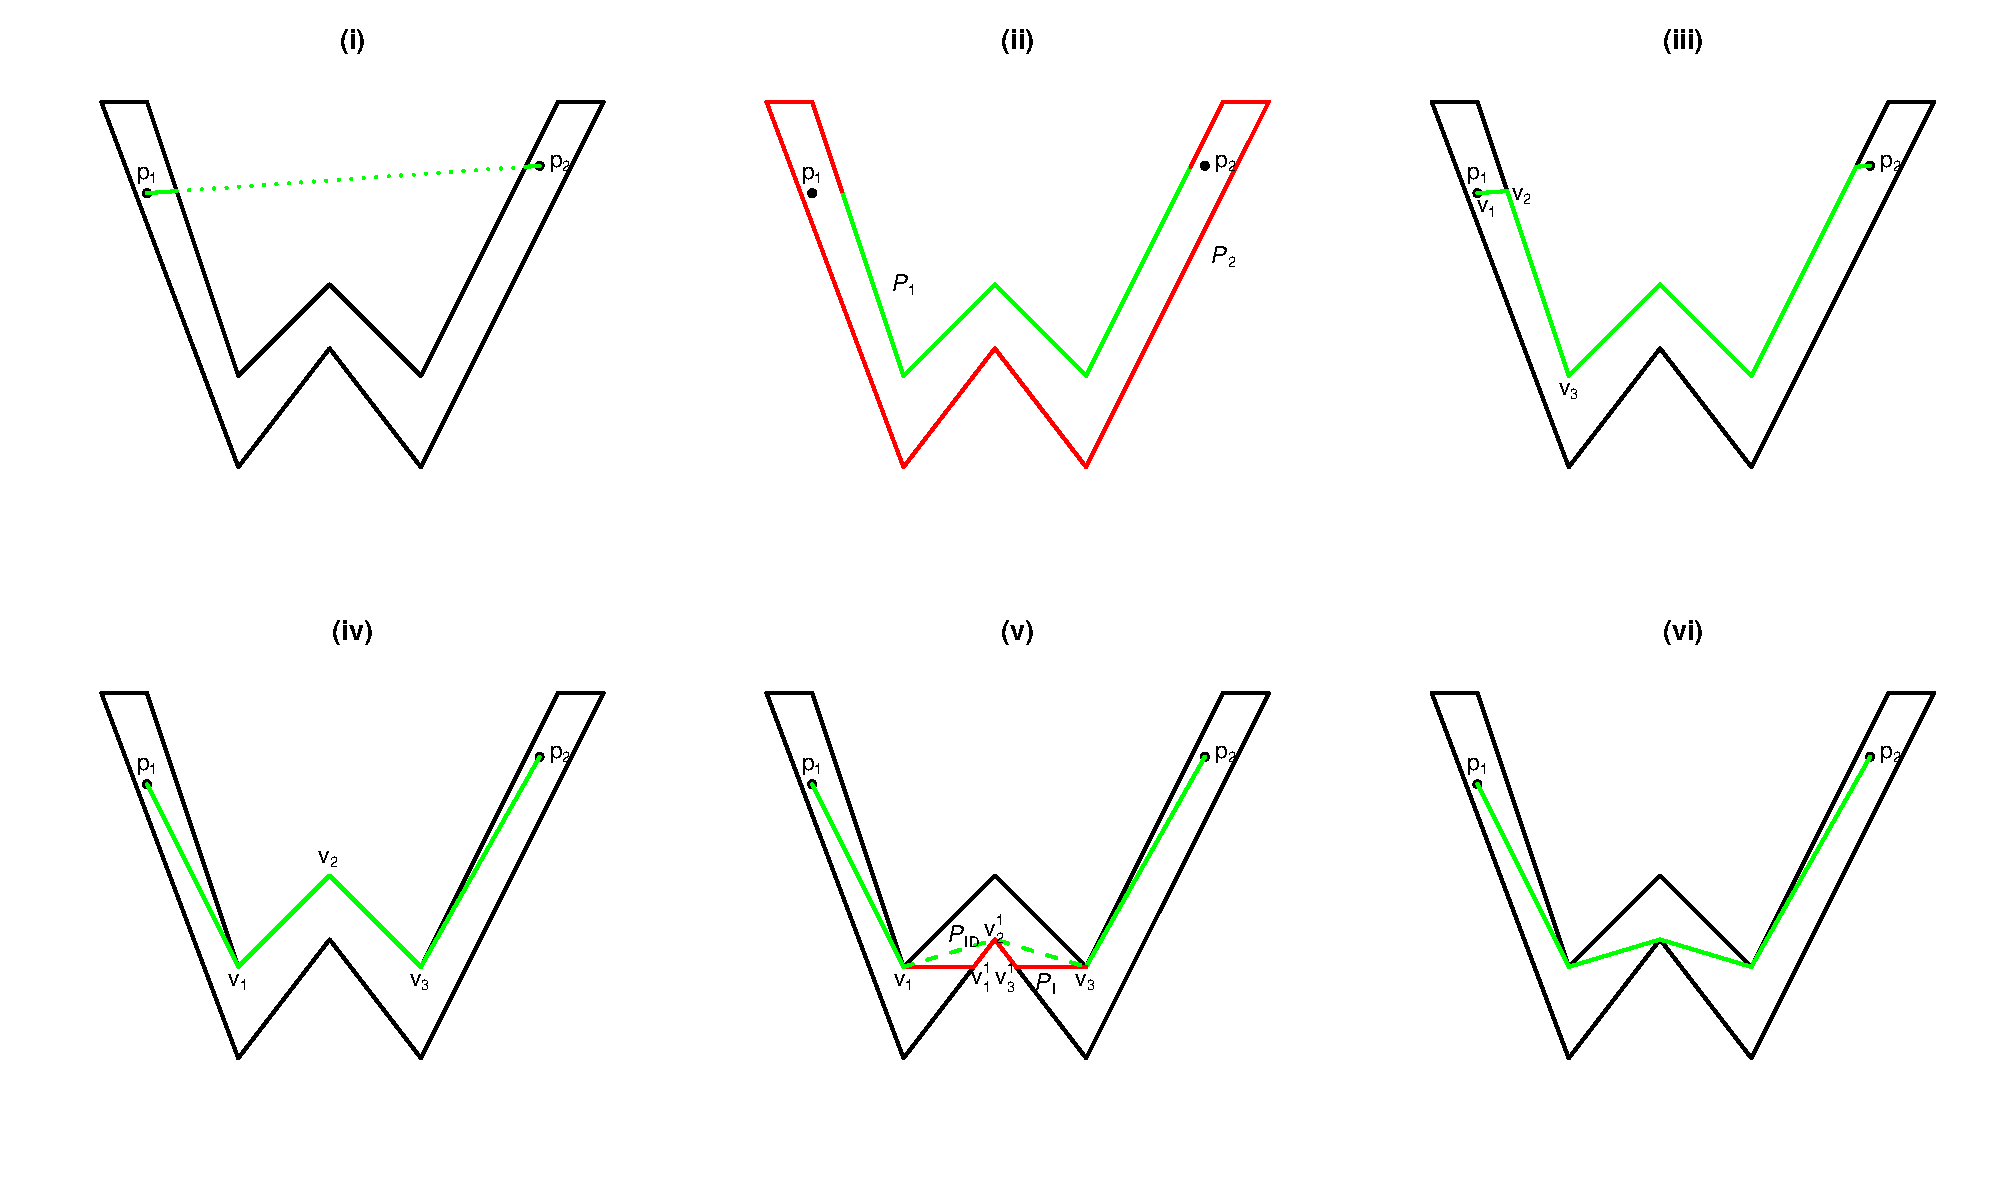
\includegraphics[width=\textwidth, trim=0in 0.5in 0in 0.25in]{figs/wdia.pdf} \\
\caption{Finding the shortest within-area path. The green lines in ($i$) to ($vi$) show the steps forming the shortest path as the algorithm progresses from initial state to final, shortest path (bottom right). See Appendix B for more details.}
\label{wdia}
% generated by figs/distanceexplanation.R
\end{figure}

Of course, if there is a direct path between $p_1$ and $p_2$ then the Euclidean distance between the points can be used and the above algorithm is not run.

Although the authors were not able to prove theoretically that the algorithm will always converge to the shortest path, it is clear at least the the algorithm will always converge (since this only requires that there be no change in the path for two consecutive iterations). Extensive simulations showed that the algorithm gave sensible results.


\subsection*{Speed improvement via partial path calculation}

It is often the case that the points for which distances are required form a grid (for example, the initial MDS grid, or prediction points). This grid setup can be exploited since there are many sets of paths that are rather similar. These paths may perhaps only differ in their final vertex. When this is the case much computational time is wasted calculating similar paths, we can exploit this problem to increase the speed of the path calculation.

By appending the points between which the within-area distance is required to either end of one of a series of pre-calculated base paths, then optimising this new path using the DELETE and ALTER steps as before,  the computational time taken to find the paths is reduced. Using base paths removes the expensive calculation in the middle of the path, where the bulk of the interactions with the boundary take place.

The algorithm is as follows, with notation and routines (INIT, DELETE, ALTER and ITER) identical to those above:
\begin{enumerate}
 \item Begin by creating a sparse grid of within the simple polygon $\Gamma$ and calculate the ($M$, say) non-Euclidean within-area paths between all pairs of points in the grid, as above. Store these paths as $\mathcal{P}_1,\ldots, \mathcal{P}_M$.
\item For each unique pairing of $p_i$ and $p_j$ in the full data set, calculate the path using one of the following:
\begin{enumerate}
\item Find a $\mathcal{P}_k$ such that the path between $p_i$ and one end of $\mathcal{P}_k$ and $p_j$ and the other end of $\mathcal{P}_k$ is Euclidean within $\Gamma$. Join $p_i$ and $p_j$ onto the appropriate ends of $\mathcal{P}_k$ and alternate between DELETE and ALTER steps until convergence.
\item If no $\mathcal{P}_k$ can be found calculate the path between $p_i$ and $p_j$ as above. 
\end{enumerate}
\end{enumerate}

Note that those paths between points in the sparse grid which are Euclidean are not stored since it is always at least as expensive to store, add to and optimise those paths then calculating them from scratch. If the required path is Euclidean anyway, then retrieving a Euclidean path, adding in $p_i$ and $p_j$, and then iterating over ALTER and DELETE steps to make it both the shortest and a Euclidean path will take longer than just creating a Euclidean path to begin with. If the path between $p_i$ and $p_j$ is non-Euclidean then the non-Euclidean part of the path must lie outside $\mathcal{P}_k$ (by definition, if $\mathcal{P}_k$ were Euclidean) and therefore will take the same number of operations to find the boundary crossing points and calculate the shortest path around the feature locally as it will to calculating the whole path from scratch.

This speed-up reduced the time to fit MDSDS to the peninsulae domain above (without MDS dimension selection) from 84 seconds to 18 seconds on a MacBook Air (2,1) with a 1.86GHz Intel Core 2 Duo processor.

This algorithm could be further improved by finding optimal starting grids. Adapting the methods described in L{\o}land and H{\o}st (2003) to approximate the distances using a triangulation, could increase performance (although perhaps at the price of accuracy).


\begin{thebibliography}{99}

\bibitem{} Gower, J. C. (1968). Adding a point to vector diagrams in multivariate analysis. \textit{Biometrika}, \textbf{55}(3), 582--585.

\bibitem{} Hart, P. E., Nilsson, N. J. and Raphael, B. (1968). A Formal Basis for the Heuristic Determination of Minimum Cost Paths. \textit{IEEE Transactions on Systems Science and Cybernetics SSC4} \textbf{4}(2), 100--107.

\bibitem{} L{\o}land, A. and H{\o}st, G. (2003). Spatial covariance modelling in a complex coastal domain by multidimensional scaling. \textit{Environmetrics} \textbf{14}(3), 307--321.

\bibitem{} Miller, D.L. (2012) \textit{On smooth models for complex domains and distances}. PhD thesis, University of Bath.

\bibitem{} Scott-Hayward, L.A.S., Mackenzie, M.L., Donovan, C.R., Walker, C.G. and Ashe, E. (under review) Complex Region Spatial Smoother (CReSS).

\bibitem{} Wang, H. and Ranalli, M.G. (2007). Low-rank smoothing splines on complicated domains. \textit{Biometrics} \textbf{63}(1), 209--217

\end{thebibliography}

\end{document}

